%\newcommand{\ans}[1]{}
\documentclass[11pt]{article}
\usepackage{fullpage,pst-all,epsfig}

\usepackage{algorithmic}
\usepackage{algorithm}

\usepackage[margin=1in]{geometry}% http://ctan.org/pkg/geometry
\usepackage{lipsum}% http://ctan.org/pkg/lipsum
\usepackage{graphicx}

\usepackage{caption}
\usepackage{subcaption}

\newcommand{\comment}[1]{}
\newcommand{\Le}{\textbf{L}}

\newcommand{\ans}[1]{\emph{Solution: #1}}
%\newcommand{\ans}[1]{}

\newcommand{\seq}[1]{ \langle #1,\cdots \, \rangle}
\newcommand{\seqi}[1]{ \langle #1 \rangle}
	
\begin{document}
\thispagestyle{empty}
\begin{center}
\def\handout{Final Examination}
\vspace*{-.75in}
{\large University of New Mexico}\\
{\large Department of Computer Science}\\
\vspace*{0.5in}
{\LARGE {\bf \handout}}\\
\vspace*{0.1in}
{\large CS 561 Data Structures and Algorithms}\\
{\large Fall, 2013}\\ [0.3in]
\end{center}
 
\vfill

\makeatletter
\long\def\hint#1{({\em Hint\/}: #1)}
% \def\@oddhead{\rm\makebox[0in][l]{CS 461 Midterm ---Fall,
% 2003}\hfil\thepage\hfil\makebox[0in][r]{Name:\rule[-0.1in]{2in}{.5pt}}}
\let\@evenhead\@oddhead
\def\@oddfoot{}
\let\@evenfoot\@oddfoot

\def\problem#1{\def\problemheading{#1}\clearpage\item{\bf #1}}

% Comment out the above 'problem' def and use the one below to get
% all the problems on a single page, instead of page break each time.
%\def\problem#1{\def\problemheading{#1}\item{\bf #1}}

\def\extrapage{\addtocounter{enumi}{-1}\clearpage\item{\bf \problemheading, continued.}}

\let\part\item
\renewcommand{\theenumii}{\alph{enumii}}
\makeatother
\parindent 0pt

\vfill
\centerline{
\Large
\begin{tabular}{|l|}  \hline
Name: \hspace*{2in} \\ \hline
Email: \hspace*{2in}\\ \hline
\end{tabular}
}
\vfill

\hrule
\begin{itemize}

\item This exam lasts 2 hours.  It is closed book and closed notes wing no electronic devices.  However, you are allowed a 1 page cheat sheet.

\item {\em Show your work!}  You will not get full credit if we cannot figure out how you arrived at your answer.  

\item Write your solution in the space provided for the corresponding problem.

\item If any question is unclear, ask for clarification.

\end{itemize}
\hrule
\vfill
\centerline{
\Large
\begin{tabular}{|c|c|c|c|}  \hline
Question & Points & Score & Grader \\  \hline\hline
1 & 20 & & \\  \hline
2 & 20 & & \\  \hline
3 & 20 & & \\  \hline
4 & 20 & & \\  \hline
5 & 20 & & \\  \hline
\hline Total & 100 & & \\  \hline
\end{tabular}
}
\vfill

\newpage

\begin{enumerate}
 

\problem{Short Answer}
 
Answer the following questions using \emph{simplest possible} $\theta$ notation.  Draw a box around your final answer.  No need to justify answers for problems on this page.
 
 \begin{enumerate}

\item ${n \choose 3} \frac{1}{n^{2}}$ \ans{$\theta(n)$}  \\ \ \\ \ \\ \ \\ \ \\ 

\item \emph{Worst case} runtime of randomized quicksort on a list of $n$ elements? \ans{$\theta(n^{2})$} \\ \ \\ \ \\ \ \\ \ \\

\item Expected number of items at the $\log n$ level of a skip list? \ans{$\theta(1)$} \\ \ \\ \ \\ \ \\ \ \\

\item Solution to the following recurrence $T(n) = 2T(n/4) + \sqrt{n}$ \ans{$\theta(\sqrt{n} \log n)$ by Master Method.}  \\ \ \\ \ \\ \ \\ \ \\

\item Solution to the following recurrence relation: $f(n) = 3f(n-1) - 2f(n-2)$. \ans{$\theta(2^{n})$ or $\theta(c_{1}2^{n} + c_{3})$.  Annihilator is $(L - 2)(L-1)$.} \\ \ \\ \ \\ \ \\ \ \\ 

\pagebreak

\item The time to determine if a weighted graph with $n$ nodes and $m$ edges has a negative cycle that is reachable from a given node.  \ans{$\theta(mn)$.  Use Bellman-Ford.} \\ \ \\ \ \\ \ \\ \ \\

\item Recall that in class we showed how to create a Dynamic table where the amortized costs for Insert and Delete were $\theta(1)$.  If an algorithm makes $\theta(n)$ calls to Insert or Delete in a table, what is the worst case cost of all of these calls?  \ans{$\theta(n)$} \\ \ \\ \ \\ \ \\ \ \\

\item What is the worst case cost of a single one of the $n$ calls in the problem above?  \ans{$\theta(n)$} \\ \ \\ \ \\ \ \\ \ \\

\item Recall that Kruskal's algorithm uses the Union-Find data structure as follows: there are $n$ calls to Make-Set, at most $2m$ calls to Find-Set and at most $n$ calls to Union.  In class, we showed that the amortized cost of each of these three operations is $O(log^{*} n)$ when there are $n$ elements in the sets.  Based on these facts, what is the amount of time Kruskals spends on Union-Find operations in the worst case?  \ans{$\theta((m+n)\log^{*}n)$} \\ \ \\ \ \\ \ \\ \ \\

\item You have computed a max flow $f$ in a network $G$ with $n$ nodes and $m$ edges, and now an edge of $G$ has its capacity increase by exactly $1$.  What is the cost of the most efficient algorithm to find a new max flow for $G$?
\ans{Compute the residual graph of $G$ and then determine whether or not there is an augmenting path in this residual graph.  The augmenting path can be found in $\Theta(m+n)$ time by using BFS from $s$.  At most $1$ augmenting path is necessary to find the new max flow since the increased capacity of the new edge can increase the value of the flow by at most $1$} \\ \ \\ \ \\ \ \\ \ \\

\end{enumerate}


\problem{Short Answer}

\begin{enumerate}

\item (10 points) Before a party, $n$ people check their hats.  The hats are mixed up during the party so that at the end of the party, each person gets a random hat.  In particular, each person gets their own hat with probability $1/n$.  What is the expected number of people who receive their own hat?

\ans{Let $X_{i}$ be $1$ if person $i$ gets their own hat and $0$ otherwise.  Let $X = \sum_{i=1}^{n} X_{i}$.  Then $E(X) = \sum_{i=1}^{n} E(X_{i}) = 1$.  So we expect $1$ person to get their own hat back.}






\pagebreak

\item (10 points) In 4-SAT problem, you are given a boolean formula, $f$, in conjunctive normal form where each clause has exactly $4$ variables, and you are asked if this formula can be satisfied.  For example, given $f = (a \lor b \lor c \lor d) \land (\lnot{a} \lor \lnot{b} \lor \lnot{c} \lor \lnot{d}) \land (a \lor \lnot{b} \lor c \lor \lnot{d}) $, you should return YES since $f$ can be satisfied (for example when $a$ and $b$ are TRUE and $c$ and $d$ are FALSE).  Show that 4-SAT is NP-HARD by a reduction from one of the following problems: SAT, 3-SAT, CLIQUE or INDEPENDENT-SET.

\ans{We show this by a reduction from 3-SAT.  Let $f$ be an arbitrary 3-CNF formula.  Create a new 4-CNF formula $f'$ from $f$ by creating a new variable $x$ and adding it to every clause of $f$.  Then add one additional clause to $f'$ that is $(\lnot{x} \lor \lnot{x} \lor \lnot{x} \lor \lnot{x})$.  Note that any assignment that satisfies $f$ can be used to satisfy $f'$: set all variables for $f'$ the same as for $f$ and set $x$ to FALSE.  Further, any assignment that satisfies $f'$ will satisfy $f$: set all variables for $f$ the same as for $f'$ and ignore the value of $x$.  Thus, $f'$ is satisfiable iff $f$ is satisfiable and so a polytime algorithm for 4-SAT gives a polytime algorithm for 3-SAT.}



\end{enumerate}


\problem{Dynamic Programming}

You are given an input string and a dictionary of words, and need to determine if the input string can be segmented into a space-separated sequence of dictionary words.  For example, given the dictionary $\{algorithms, data, structure, i, love, snow\}$ and the input string $``ilovealgorithms''$, you should output TRUE since the input can be segmented as ``i love algorithms''.  

Assume you have a function ``InDictionary(x)'' that returns TRUE iff a string $x$ is in the dictionary, and this function runs in $O(1)$ time.  As input, you are given a string $s$, which is represented as an array of length $n$, i.e. $s = s[1,\ldots,n]$.   Define a function $f$ such that $f(i)$ is TRUE iff the substring $s[1..i]$ can be segmented for $0 \leq i  \leq n$.  Define $s[0]$ to be the empty string.

\begin{enumerate}

\item (15 points) Write a recurrence relation for $f$.
\ans{Base case: $f[0] = TRUE$.  For $1 \leq i \leq n$,  $f(i) = TRUE$ iff there exists some $j$, $0 \leq j < i$, such that $f(i-j)$ is TRUE and InDictionary(s[j+1, \ldots, i]])} \\ \ \\ \ \\ \ \\ \ \\ \\ \ \\ \ \\ \ \\ \ \\


\item (5 points) Describe in 1-3 sentences (no need for pseudo-code) how you would create a dynamic program based on your recurrence to find the value of $f(n)$.  What are the time and space costs of your algorithm?

\ans{Create an array of size $n$ to store the values of $f$.  Compute values of $f$ from left to right in this array.   Return $f(n)$.  Time is $\theta(n^{2})$.  Space is $\theta(n)$.}

\end{enumerate}



\problem{Max Flow}

\begin{figure}[h]
\begin{center}
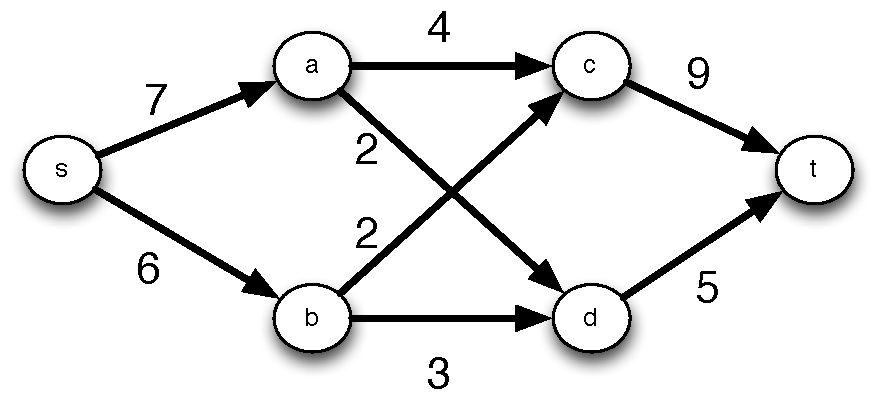
\includegraphics[scale=0.4]{nf.pdf} 
\caption{}
\label{f:path}
\end{center}
\end{figure}

\begin{enumerate}

\item (3 points) Consider the above network (the numbers are edge capacities).  Find the max flow, $f$,  and a min cut in this network.  
\ans{The flow The cut is $S = \{s,a,b\}$ and $T = \{c,d,t\}$ } \\ \ \\ \ \\ \ \\ \ \\ \ \\ \ \\ \ \\ \ \\ \ \\

\item (3 points) Draw the residual graph $G_{f}$ (along with its edge capacities). In this residual network, mark the vertices reachable from $s$ and the vertices from which $t$ is reachable. 
\ans{\begin{figure}[h]
\begin{center}
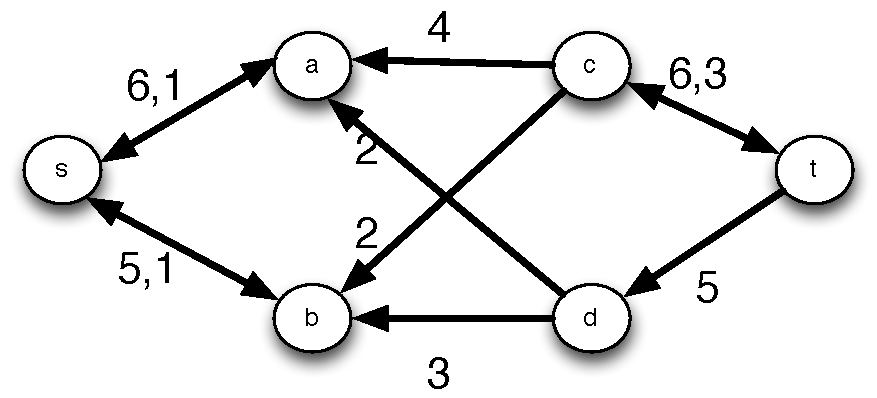
\includegraphics[scale=0.4]{nf-residual.pdf} 
\caption{}
\label{f:path}
\end{center}
\end{figure}} \\ \ \\ \ \\ \ \\ \ \\ \\ \ \\ \ \\ \ \\ \ \\

\pagebreak

\item (3 points) An edge of a network is called a \emph{bottleneck} edge if increasing its capacity results in an increase in the maximum flow. List all bottleneck edges in the above network. \ans{(a,c) and (b,c)}  \\ \ \\ \ \\ \ \\ \ \\ \ \\ \ \\ \ \\ \ \\ 

\item (3 points) Give a very simple example (containing at most four nodes) of a network which has no bottleneck edges. All capacities on your network should be finite.\ans{Nodes are s,a,b,t.  There are $4$ edges, each with capacity $1$: (s,a), (a,t), (s,b), (b,t)}  \\ \ \\ \ \\ \ \\ \ \\

\pagebreak

\item (8 points) Give an efficient algorithm to identify all bottleneck edges in a network. (Hint: Start by running the usual network flow algorithm, and then examine the residual graph.) \ans{Run the network flow algorithm and find the final residue network. For each edge in the original graph, check in the residual network whether the source node of the edge is reachable from s and the target node of the edge can reach t. You can use a depth first search algorithm to check the reachability. If the paths from s to u and v to t exist, then edge (u, v) is a bottleneck edge. In fact, you do not have to run the depth first search for each edge. Instead you can run one depth first search for s on the residue network and another for t on the reverse residue network (all edges reversed) and keep the reachable nodes.
} \\ \ \\ \ \\ \ \\ \ \\

\end{enumerate}


%\extrapage


\problem{Square in Matrices}

You are given a $m$ by $n$, matrix, $M$, where each cell is either a ``1''  or ``0''.    Your goal is to find a maximum size square sub-matrix with all 1's.   

\begin{verbatim}
0 1 1 0 1
1 1 0 1 0
0 1 1 1 0
1 1 1 1 0
1 1 1 1 1
0 0 0 0 0
\end{verbatim}

For example, the above matrix has a maximum size square matrix that is 3 by 3, with bottom right corner at $M(5,4)$.  Give an efficient algorithm to solve this problem.  Compute the time and space costs of your algorithm.

\ans{Let $S(i,j)$ be the size of the largest square matrix of all 1's whose bottom right corner is $M(i,j)$.  We can write a recurrence relation for $S(i,j)$ as follows.  If $i<1$ or $j<1$, then $S(i,j) = 0$.  Else if $M(i,j) = 0$ then $S(i,j) = 0$.  Otherwise if $M(i,j) = 1$, then $S(i,j) = 1 + \min(S(i,j-1), S(i-1,j-1), S(i-1,j)$.  We create this $S$ array moving from left to right and top to bottom.   We also keep track of the maximum value, $M$, in the $S$ array and the location $L_{M}$ where this maximum value occurs.  After filling in all entries of $S$, we return that the largest all $1$ submatrix is of size $M$ by $M$ and has bottom right corner at location $L_{M}$.  This algorithm take $O(mn)$ time.}

 
 
 
 \extrapage


\end{enumerate}

  
  
 
  \end{document}
 
 
   \problem{Recurrences and Asymptotics}
 
 Remember that when the base case for a recurrence is not explicitly given, assume that it is constant for inputs of constant size.
 
 \begin{itemize}
 
 \item Consider the recurrence $f(0) = 1$, $f(n) = \sum_{i=0}^{n-1} f(i)$.  Prove that the solution to this recurrence is $\theta(2^{n}$)
 
 \ans{This is a straightforward proof by induction.}
 \ \\ \ \\  \ \\ \ \\ \ \\  \ \\ \ \\ \ \\  \ \\ \ \\ \ \\  \ \\ \ \\ \ \\  \ \\ \ \\ \ \\  \ \\

\item Solve the following recurrence: $f(n) = 4f(n-1) - 4f(n-2) + 2^{n}$.  Do not solve for the constant coefficients
\ans{$(L^{2}-4L+4) = (L-2)^{2}$ annihilates the homogeneous part and $(L-2)$ annihilates the non-homogeneous part.  So the annihilator is $(L-2)^{3}$ and hence the solution is $(c_{1}n^{2} + c_{2} n + c_{3}) 2^{n}$}
 \ \\ \ \\  \ \\ \ \\ \ \\  \ \\ \ \\ \ \\  \ \\ \ \\ \ \\  \ \\

\pagebreak


\item Solve the following recurrence: $f(n) = f(n/2) + f(n/4)$.  Do not solve for the constant coefficients.  If an algorithms runtime is given by this recurrence, how would it compare with algorithms with runtimes of $\theta(2^{n})$, $\theta(n)$, $\theta(\sqrt{n})$?

 \ans{Let $2^{i}=n$ and $F(i) = f(2^{i})$.  Then we get a transformed recurrence: $F(i) = F(i-1) + F(i-2)$, whose solution is  $F(i) = c_{1} \phi^{i} + c_{2} \hat{\phi}^{i}$. Reverse transforming this solution, and using the fact that $i = \lg n$ we get  
 $f(n) = n^{\lg \phi} + n^{\lg \hat{\phi}}$.  This solution is approximately $\theta(n^{.694})$, so it is better than linear but worse than square root run time.}
 \ \\ \ \\  \ \\ \ \\ \ \\  \ \\ \ \\ \ \\  \ \\ \ \\ \ \\  \ \\
 
 \end{itemize}

\problem{Heaps and Sorting}

Professor Humbert claims to have invented a new Max-Heapify function for heaps that runs in $O(\lg \lg n)$ time.  Moreover, Humbert claims that his new Max-Heapify function is completely comparison based, i.e. the only way it ever compares two keys is with the $\leq$ operator.  Could Humbert be right?

\ans{No.  If such a Max-Heapify function existed, we could plug it into heap sort and use if to do comparison-based sorting in $\Theta(n\lg \lg n)$ time. }

 \ \\ \ \\ \ \\  \ \\ \ \\ \ \\  \ \\ \ \\ \ \\  \ \\

Prove that the following algorithm correctly sorts a list of $n$ elements by induction on $n$.  Don't forget to include the base case, inductive hypothesis and inductive step.
\begin{verbatim}
SillySort(A, i, j){
  Let n = j - i + 1;                   // n is the number of elements to sort
  If n <= 1 then return;          //nothing to sort
  If n == 2                              // only two elements to sort
    then
      if A[i] > A[j], swap A[i] and A[j]
  else                                     // more than two elements to sort                    
     SillySort(A,i+n/2,j);         //SillySort the last n/2 elements of A
     SillySort(A,i,i+n/2);    //SillySort the first n/2+1 elements of A
     SillySort(A,i+1,j)             //SillySort the last n-1 elements of A
 }
\end{verbatim}

\extrapage

\ans{Prove by induction on the size of L.  Need to first prove that the minimum element in the array winds up in the first position.}

\problem{Data Structures}

\begin{itemize}

\item Imagine that in a red black tree, the rule that a red node must have two black children is relaxed to the rule that a red node must have at least one black child.  All other rules remain the same.  What is now the maximum asymptotic height that a red black tree with $n$ nodes can have?  Give an example or proof as necessary to justify your claim.

\ans{The tree can now have $\theta(n)$ height.  Imagine one branch where all the nodes are red except for the root, and one child of each node on the branch - the final node in this branch has two black children.}

\pagebreak

\item Imagine you have a ``blacklist'' of $n$ messages that are spam.  When a new message arrives in your mail queue, you want to test it to see if it's a message in your black list.  However, space is at a premium and so you don't want to have to store all $n$ messages in memory (assume each message is many bits in length).  Answer the following questions with asymptotic notation.  Hint: Assume that you have a hash function that maps strings of any size to integers that are essentially random.
\begin{itemize}
\item What is the minimum number of bits of space to ensure that you can test if new messages are in the blacklist and get false positive with probability no more than $1/100$?  What is the time needed to test if a message is in the blacklist in this case?
\item How many bits do you need if you want the probability of false positives to be no more than $1/n$?  What is the time to test membership in this case?
\end{itemize}
\ans{Use a Bloom filter.  You need $\theta(n)$ bits and $\theta(1)$ time in the first case (since $k = \theta(1)$).  In the second case, you need 
$\theta(n \lg n)$ bits (since $m$ must be $n \lg n$) to get probability of false positives less than $1/n$; you need $O(\lg n)$ time since $k$ is $O(\lg n)$}

\end{itemize}

 \problem{Probability}
 
 \begin{itemize}
 \item \emph{Bad Santa II: Mr. Kringle's Revenge:} Consider the Bad Santa problem from hw1 with the following change.  The child is allowed to take $2$ passes over the sequence of boxes if necessary, but still needs to find just one present before stopping.  However, Santa can secretly hide the presents again after the first pass of the child.  Describe and analyze an algorithm for this new problem that minimizes the expected number of boxes opened.  Hint: The problem is now much easier than the hw problem.
 
 \ans{The algorithm: In this first pass, choose $\log n$ boxes uniformly at random and open those.  In the second pass, just open all boxes from let to right until finding a present.  The expected number of boxes opened is no more than $\log n + (1/n)n$, since the probability of getting to the second pass is only $(1/2)^{\log n} = 1/n$.  Thus the expected number of boxes opened is $O(\log n)$.}
 
 \pagebreak
 
 \item \emph{Closest Points:} Imagine $n$ points are distributed uniformly at random on a circle with circumference $1$.  Show that the expected number of pairs of points that are within distance $\theta(1/n^{2)}$ of each other is greater than $1$ (note that this implies that the smallest distance between two points is likely $O(1/n^{2})$).  Hint: Partition the circle into $n^{2}/k$ regions of size $k/n^{2}$ for some constant $k$; then use the Birthday paradox to solve for the necessary $k$.
 \ans{Think of the regions as bins and the points as balls.  The probability that two points fall in the same region is $k/n^{2}$.   Let $X_{i,j}$ equal $1$ if points $i$ and $j$ fall in the same region and $0$ otherwise and let $X$ be the sum over all $n \choose 2$ values $i$ and $j$ of $X_{i,j}$.  Using linearity of expectation, $E(X) = {n \choose 2}k/n^{2}$.  Thus, for some $k$, e.g. $k\geq 3$, we would expect at least one pair of balls to fall in the same bin.}

\end{itemize}


 \problem{Are you Smarter than a 561 Student?}
 
You are competing in the popular game show ``Let's Make a Dynamic Program'' with another player.  You and your opponent both start with $0$ dollars.  If you reach (or exceed) $n$ dollars before your opponent, you win $n$ dollars; if your opponent reaches (or exceeds) $n$ dollars before you, you win nothing; and if you both reach (or exceed) $n$ dollars at the same time, you both win $n$ dollars.  In each turn, you get to choose the level of difficulty of the next question asked, where this difficulty is represented by an integer $k$ between $1$ and $n$.  If you answer the question correctly, you get $k$ dollars, otherwise your opponent gets $k$ dollars.  Note that you are always in control throughout the entire game of the difficulty level of the question asked.
 
Through careful study of the game you have been able to determine the probability $p_{i}$ for $i$ between $1$ and $n$, which is the probability that you will answer a question of difficulty $i$ correctly.

\begin{itemize}

\item Consider the greedy algorithm where you always choose a question of difficulty level $i$ for $i$ maximizing $i*p_{i} - i*(1-p_{i}) = i(2p_{i}-1) $.  Is this an optimal algorithm?  Hint: Is it ever better to make a long shot bet because the probability of success from multiple short bets is small.  In particular,think about the case where your opponent has $n-1$ dollars and you have $0$.


\ans{Greedy is not optimal.  Consider the case where $p_{1} = 1/4$, $p_{n} = 1/5$ and for all other $i$, $p_{i} = 0$.  Then $1$ is the difficulty level maximizing the expected difference between you and your opponent, since $1p_{1} - 1q_{1} = -1/2$ and $np_{n} - nq_{n} = -(3/5)n$.  Assume further that your opponent has $n-1$ dollars and you have $0$ dollars.   If you choose a difficulty of $n$, you have the chance of jumping ahead of your opponent to victory, which happens with probability at least $1/5$.  In contrast, the probability of success by following the greedy strategy, where you just keep choosing difficulty of $1$ will only be $(1/4)^{n}$, which is exponentially small in $n$.}

\pagebreak

\item Let state $(i,j)$ be the state where you have $i$ dollars and your opponent has $j$ dollars.  Note that if you choose the difficulty level to be $k$ at that state, you have probability $p_{k}$ of going to state $(i+k,j)$ and probability $(1-p_{k})$ of going to state $(i,k+jj)$.  Now let $e(i,j)$ be your expected winnings if you have $i$ dollars and your opponent has $j$ dollars and you play optimally.  Write a recurrence relation for the value $e(i,j)$.  Note: You will find it useful to consider $i$ and $j$ values that range from $0$ to $2n-1$.  Hint: Use expected values for simpler subproblems and the probabilities $p_{i}$ described above to compute $e(i,j)$.  Don't forget the base case(s).

\ans{Base Cases: $e(i,j) = n$ for all $j \geq n$.  $e(i,j) = 0$ for all $i \geq n$ and $j < n$.  \\ Recurrence:  for other values of $i$ and $j$,
 $e(i,j) = max_{1 \leq k \leq n} p_{k} e(i+k,j) + (1-p_{k}) e(i,j+k)$}

\pagebreak


\item Give the pseudocode for computing the value $e(0,0)$, which gives you your expected winnings if you play this game optimally.
\ans{Basically, need to fill in the base case first of a n by n array and then fill in the remaining values from bottom up and right to left}
  
\pagebreak 

\item What if the game is changed as follows.  You still select the difficulty level $k$, but after your selection, both you and your opponent have the chance to write down the answer to the question.  Whoever gets the answer correct wins $k$ dollars (note that both of you may win now).  There is no penalty for a wrong answer.  The probability that you answer a question of difficulty $k$ correctly is $p_{k}$ and the probability that your opponent answers correctly is $q_{k}$.   Can you still solve this new problem using dynamic programming?  If so, give a recurrence and describe how to change the algorithm.  If not, describe why not.

\ans{It is still possible.  The base case for the recurrence is the same as before.  The new part of the recurrence is determined by following equation for fixed $k$:
$e(i,j) =  (p_{k}q_{k} e(i+k,j+k) + (1-p_{k})q_{k}e(i,j+k) + p_{k}(1-q_{k})e(i+k,j) + (1-p_{k})(1-q_{k}) e(i,j)$.  Note that $e(i,j)$ appears on both the left and right side of this equation, which at first seems to cause problems in formulating a recurrence; however, it is still possible to isolate $e(i,j)$ on the left side.  Then it is possible to get a proper recurrence by taking the maximum over all possible values of $k$.  The recurrence and pseudocode is left as an exercise.}
  
 \end{itemize}
  
  \end{enumerate}
  

 
 
 \problem{Borges Library - determining if all the books in a given room are the same}
1) Create a Bloom Filter for all the books in the room
 
2) How to compare two rooms quickly to determine if they have the same set of books or not.


 
 
\problem{Data Structure Problem (BST, skip list, etc, heap)}
 
 
 
 \problem{Bday}
  
 \problem{Hafts}
 
 
 \problem{Skip Lists}
 
 \begin{itemize}
 \item How would you merge two skip lists?
 \item How would you find the $i$-th element in sorted order
 
\end{itemize}

 
 
\problem{Search Trees}

Consider a tree with the following properties:

\begin{itemize}
\item Each internal node has exactly three children
\item The heights of the subtrees rooted at each child differ by at most $1$.
\end{itemize}

What is the maximum height of such a tree containing $n$ nodes?

Hint: Write a recurrence relation for the maximum number of nodes as a function of the height and then solve for the height.  Show your work!

\ans{Let $T(h)$ be the maximum number of nodes in a tree of height $h$.  Then $T(h) = T(h-1) + 2 T(h-2) + 1$.  $(\Le^{2}-\Le - 2) = (\Le -2)(\Le +1)$ annihilates the homogeneous part and $\Le - 1$ annihilates the non-homogeneous part.  Thus, the solution is of the form $T(h) = c_{1}2^{h} + c_{2} + c_{3} (-1)^{h}$.  Let $n$ be the number of nodes in the tree.  We know that $n \geq T(h)$ and so $n \geq c_{1}2^{h} + c_{2} + c_{3} (-1)^{h}$.  If we let $c = c_{2} - c_{3}$, we can say that, $n \geq c_{1} 2^{h} + c$.  Taking logs of both sides, we have that $\log n \geq h \log (2c_{1}) + \log c$.  This implies that $h \leq 1/(log(2c_{1}))(\log n - \log c)$.  The right hand side is $O(\log n)$.  Thus, $h$ is $O(\log n)$.}

\problem{Hash Tables and Probability}

Assume we hash $n$ items into a hash table with $n$ bins using a good hash function i.e. each item is hashed to a bin chosen independently and uniformly at random.  Give a good upper bound on the number of empty bins.  Solve for the constants in your upper bound i.e. do not use asymptotic notation.

Hint: Use the fact that $1-x \leq e^{-x}$ for all $x$.

\ans{Let $X_{i}$ be an indicator random variable which is $1$ if the $i$-th bin is empty and is $0$ otherwise.   Then note that $E(X_{i})$ equals the probability that the $i$-th bin is empty.  This is the probability that the $n$ items do not fall in bin $i$.  The probability that a single item does not fall in bin $i$ is exactly $1 - 1/n$.  Since the items are all hashed independently, the probability that \emph{no} item hashes into bin $i$ is exactly $(1-1/n)^{n}$.  Using the hint, note that  $(1-1/n)^{n} \leq (e^{-1/n})^{n} = e^{-1}.$  Let $X$ be a random variable giving the number of empty bins and note that $X = \sum_{i=1}^{n} X_{i}$.  Using linearity of expectation, we see that $E(X) = E(\sum_{i=1}^{n} X_{i}) = \sum_{i=1}^{n} E(X_{i}) \leq n/e$.  Thus the expected expected number of empty bins is at most $n/e$.  This is actually a pretty tight upper bound as $n$ gets large.}

\problem{Divide and Conquer}

Imagine that after graduating from UNM, you start your new job at the exciting investment banking firm SELLOUT, Inc.  The firm if faced with the following problem: they have an array of the predicted prices of a stock over $n$ days and they want to determine, using this array, exactly one day to buy the stock and one day to sell the stock in order to maximize their profit.

The problem can be formally stated as follows.  You are given an array $A$ of $n$ numbers.  You want to choose indices $1 \leq i < j \leq n$ such that $A[j] - A[i]$ is maximized over all such indices.  Give an $o(n^{2})$ algorithm to solve this problem.

\ans{Use Recursion!  Recursively find the pair of indices $i_{l}$ and $j_{l}$ on the left half of the array such that $i_{l} < j_{j}$ and $A[j]-A[i]$ is maximized over all such pairs.  Find a similar pair $i_{r}$ and $j_{r}$ on the right half of the array.  Now find $x$, the index of the element with smallest value on the left half and $y$, the index of the largest element on the right half.  Finally, return 
max($A[j_{l}] - A[i_{l}]$, $A[j_{r}] - A[i_{r}]$, $A[y] - A[x]$).  The run time of this algorithm is given by the same recurrence as for merge sort $T(n) = 2T(n/2) + n$, whose solution is $n \log n$.  Note that we can get an even faster algorithm than this using dynamic programming. Also there is another $O(n \log n)$ solution that makes use of a heap or BST.}

\end{enumerate}

\end{document}





% \item {\bf True or False}:  In a max-heap, the element with smallest key is always at the
% rightmost leaf node of the heap? \ans{F: it's always at a leaf node
% but not necessarily the rightmost leaf node}
% \item {\bf True or False}:  Bubblesort requires $O (n)$ extra space (not counting the space
% to store the array to be sorted)? \ans{F: it takes $O (1)$ extra space}
% \item {\bf True or False}:  $1/\log n$ is $o (1)$? \ans{T}
% \item {\bf True or False}:  $\log \sqrt{n}$ is $\Theta (\log n)$?
% \ans{T: since $\log \sqrt{n} = 1/2\log n$}
% \item {\bf True or False}:  $2^{n-1}$ is $o (2^{n})$?\ans{F: since $2^{n-1}=1/2*2^{n}$}
% \problem{Annihilators}\\

% Consider the recurrence $T (n) = 2T (n-1) - T (n-2) + 4$, $T (0)=0$, $T (1)=0$.
% Solve this recurrence \emph{exactly} using annihilators.  Don't forget
% to check your answer.

% \ans{Consider the homogeneous part first.  Let $T_{n} = 2T (n-1) - T
% (n-2)$, and $T = \seqi{T_{n}}$.  Then
% \begin{eqnarray}
% T & = & \seqi{T_{n}}\\
% \Le T & = & \seqi{T_{n+1}}\\
% \Le^{2} T & = & \seqi{T_{n+2}}
% \end{eqnarray}
% Since $\seqi{T_{n+2}} = \seqi{2T_{n+1}-T_{n}}$, we know that
% $\Le^{2}T-2\Le T + T = \seqi{0}$, and thus $\Le^{2}-2\Le +1 = (\Le -1)
% (\Le -1)$ annihilates $T$.  Further we know that $(\Le -1)$
% annihilates the non-homogeneous part.  Thus the annihilator of the
% whole sequence is $(\Le -1)^{3}$.  Thus $T (n)$ is of the form:
% \[
% T (n) = c_{1}n^{2}+c_{2}n+c_{3}
% \]
% We know:
% \begin{eqnarray}
% T (0) = 0 & = & c_{3}\\
% T (1) = 0 & = & c_{1} + c_{2}\\
% T (2) = 4 & = & 4 c_{1} + 2c_{2}
% \end{eqnarray}
% so $c_{1}=2$, $c_{2}=-2$, $c_{3}=0$ and thus
% \[
% T (n) = 2n^{2}-2n
% \]
% Check: $T (3) = 2*4-0+4=12$ and $2*9-6=12$.}




% \problem{Substitution Method}\\
% Consider the following recurrence: $$T(n) = T(n-1) + T(n-2) - n + 3,$$
% where $T(1) = 1,T(2)=2$.\\ \ \\ Show that $T(n) = n$ by induction.
% Include the following in your proof: 1)the base case(s) 2)the
% inductive hypothesis and 3)the inductive step.

% \ans{Base Case: T(1) = 1.\\Inductive Hypothesis: For all $j<n$, T(j) =
% j\\Inductive Step: We must show that $T(n)=n$, assuming the inductive
% hypothesis.  
% \begin{eqnarray}
% T(n) & = & T(n-1) + T(n-2) - n + 3\\
% T(n) & = & (n-1) + (n-2) - n + 3\\
% T(n) & = & n
% \end{eqnarray}
% where the inductive hypothesis allows us to make the replacements in
% the second step.}

% \item {\bf True or False}: If $X$ and $Y$ are sequences that both
% begin with the character $a$, then some longest common subsequence of
% $X$ and $Y$ begins with the character $a$. \ans{True}
 \pagebreak

\item (5 points) Your boss wants to create the following data structure in the comparison model and to name it after himself, the \emph{Merkle}.  A Merkle has the following operations and properties on it.  BuildMerkle takes an arbitrary array and builds a Merkle from it in $O(n)$ time.  The resulting Merkle will provide the following operations.  FindMin (resp. FindMax) will return the minimum (resp. maximum) element and run in $O(\log n)$ time.  Successor(x) (resp. Predecessor(x)) return the next largest (resp. smallest) element in the Merkle after the element $x$, and both of these operations run in $O(1)$ time.  Intuitively, your boss wants you to combine the nice properties of the heap with the nice properties of a data structure like skip lists.  Can you immortalize your boss's name in CS textbooks by creating this data structure?

\ans{No.  This would allow sorting in $O(n)$ time.  To show this, first build the Merkle from an unsorted array, then find the minimum element and keep calling successor}



\pagebreak

In this problem, you will modify count-min sketches so that they handle negative counts.  As in class, assume you are presented with a stream of tuples of the form $(i_{t},c_{t})$, except now $c_{t}$ may be either a negative or positive integer.  The data structure you will use will consist of two count-min sketches, a positive count-min sketch for positive counts and a negative count-min sketch for negative counts.  In particular, each of the two sketches will use $m$ counters and $k$ hash functions, where all hash functions can be assumed to be independent.  If $c_{t}$ is positive, in the positive count-min sketch (positive sketch for short),  for each $1 \leq a \leq k$, $C_{a,h_{a}(i)}$ will be incremented by $c_{t}$.  If $c_{t}$ is negative, in the negative sketch, for each $1 \leq a \leq k$, $C_{a,h_{a}(i)}$ will be incremented by $-c_{t}$.   The estimate of the count of an item, $i$ at time $T$ is $m^{+}(i,T) - m^{-}(i,T$, where $m^{+}(i,T)$ is the value of the smallest counter associated with $i$ in the positive sketch and $m^{-}(i,T)$ is the value of the smallest counter associated with $i$ in the negative sketch.  As in class, let $Count(i,T)$ be the true count of item $i$ in the stream up to time $T$.  Also assume that $k = m \epsilon/e$ for the positive sketch and for the negative sketch.
 
 \item (7 points) Give a good bound on the probability that the following holds:\\
 $$ Count(i,T) - \epsilon \sum_{i=1}^{T} |c_{i}| \leq m(i,T) \leq Count(i,T) + \epsilon \sum_{i=1}^{T} |c_{i}| $$
 Please prove your bound.
 
 
 \ans{Let $S^{+}_{T}$ be the sum of all the positive counts in the stream up to time $T$.  For the positive sketch, we know that $Pr(Z_{j}> \epsilon S^{+}_{T}) \leq e^{m\epsilon/e}$, where $Z_{j}$ is the amount the min counter associated with $i$ in the positive sketch is incremented by items other than $i$.  Let $S^{-}_{T}$ be the sum of the absolute values of the negative counts in the stream up to time $T$.  Then we also know using the analysis in class that for the negative sketch, $Pr(Z'_{j}> \epsilon S^{-}_{T}) \leq e^{m\epsilon/e}$, where $Z'_{j}$ is the amount the min counter associated with $i$ in the negative sketch is incremented by items other than $i$.   A simple union bound on these two inequalities shows that $Pr(Z_{j}> \epsilon S^{+}_{T} \textrm{ or } Z'_{j}> \epsilon S^{-}_{T}) \leq 2 e^{m\epsilon/e}$.  Thus, we can see that $Pr(Z_{j} + Z'_{j} > \epsilon \sum_{i=1}^{T} |c_{i}|) \leq  2 e^{m\epsilon/e}$.  Thus the probability the approximation bound given holds is at least $1 - 2 e^{m\epsilon/e}$. }

\pagebreak

\item  (7 points) Now imagine you are given a constant number of data streams $D_{1}, D_{2}, \ldots, D_{c}$ and weights associated with them $w_{1}, w_{2}, \ldots w_{c}$ that may be positive or negative real numbers.  For each item $i$, at time $T$, define $Count(i,T)$ to be the weighted sum of the count values seen in all data streams up to time $T$, where a count value seen in stream $i$ is weighted by $w_{i}$.  Assume now that all count values seen are positive.  Describe a data structure based on count-min sketches that can approximate $Count(i,T)$.  How much memory does your data structure use? How closely can you approximate $Count(i,T)$ and with what probability?  Please justify your answers.  For consistency in notation, please let $S(i,j,T)$ be the sum of the counts of item $i$ in stream $j$ up to time $T$.

\ans{The basic idea is to use $c$ different count min-sketches and let $m(i,T)$ be the weighted sum of the min value in each of them associated with the item $i$.  The total memory used is $cm$.  A union bound over the $c$ different data streams can establish the following guarantee with probability $1-c e^{m\epsilon/e}$:
 $$ Count(i,T) - \epsilon \sum_{j=1}^{c} |w_{j}| S(i,j,T) \leq m(i,T) \leq Count(i,T) + \epsilon \sum_{j=1}^{c} |w_{j}| S(i,j,T) $$}


\end{enumerate}
 
 \item You are given a bipartite graph $G = (V,E)$, with nodes on the left side, $L$, representing interns and nodes on the right, $R$, representing hospitals.  There is an edge from an intern node, $x$, to a hospital node, $y$ iff the intern x is willing to be assigned to hospital $y$.  As in the homework, assume that for all $S \subseteq L$, $|N(S)| \geq |S|$.   

What is the runtime of the fastest algorithm to find a perfect matching in $G$ (in terms of $|V|$ and $|E|$)?  You should only use algorithms discussed in this class.

\ans{We create a new graph $G'$ with source $s$ and sink $t$.  There is an edge from $s$ to each node in $L$ with capacity $1$ and an edge from each node in $R$ to $t$ with capacity $1$.  Then for every edge $(x,y) \in E$, there is an edge from $x$ to $y$ with capacity $1$.  There are thus $O(E)$ edges and $O(|V|)$ nodes, all capacities are $O(1)$ and $f* = O(|V|)$.  Using the ``Short Pipe'' algorithm, we can find a max flow in $G'$ and thus a perfect matching in $G$ in time $O(|E|^{2} \log |E| \log |V|)$}


 
